\chapter{Introduction to \OM}\label{cha_int}

This chapter briefly introduces \OM concepts and notions that are referred to in the rest
of this document.

\section{\OM Architecture}\label{sec_om-arch}

\begin{figure}\centering
  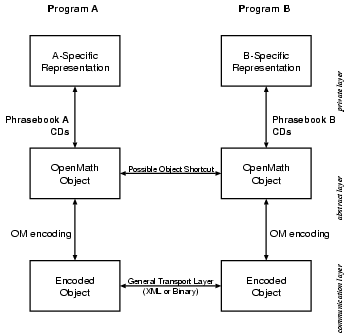
\includegraphics{om-arch}
  \caption{The \OM Architecture}\label{fig_om}
\end{figure}

The architecture of \OM is described in \ref{fig_om} and summarizes the interactions among
the different \OM components.  There are three layers of representation of a mathematical
object. The first is a private layer that is the internal representation used by an
application.  The second is an abstract layer that is the representation as an \OM object.
Note that these two layers may, in some cases, be the same.  The third is a communication
layer that translates the \OM object representation into a stream of bytes. An application
dependent program manipulates the mathematical objects using its internal representation,
it can convert them to \OM objects and communicate them by using the byte stream
representation of \OM objects.


\section{\OM Objects and Encodings}\label{sec_intro-obj}


\OM objects are representations of mathematical entities that
can be communicated among various software applications in a
meaningful way, that is, preserving their
\textquote{semantics}.

\OM objects and encodings are described in detail in \ref{cha_obj} and \ref{cha_enco}.



The standard endorses two encodings in \XML and binary
formats.
At the time of writing, these are the encodings
supported by most existing \OM tools and applications,
however they are not the only possible encodings of \OM
objects. Users who wish to define their own encoding
, are free to
do so provided that there is
a well-defined correspondence
between the new encoding and the abstract model defined in \ref{cha_obj}. 





\section{Content Dictionaries}\label{sec_intro-cd}


Content Dictionaries (CDs) are used to assign informal and formal
semantics to all symbols used in the \OM objects. They define the
symbols used to represent concepts arising in a particular area of
mathematics.


The Content Dictionaries are public, they represent the actual
common knowledge among \OM applications.  Content Dictionaries fix
the \textquote{meaning} of objects independently of the
application.  The application receiving the object may then recognize
whether or not, according to the semantics of the symbols defined in
the Content Dictionaries, the object can be transformed to the
corresponding internal representation used by the application.

\section{Additional Files}\label{sec_addnfiles} 
Several additional files are related to Content Dictionaries.  Signature Dictionaries
contain the signatures of symbols defined in some \OM Content Dictionary and their format
is endorsed by this standard.

Furthermore, the standard fixes how to define a specific set of Content Dictionaries as a
CDGroup.

Auxiliary files that define presentation and rendering or that are used for manipulating
and processing Content Dictionaries are not discussed by the standard.

\section{Phrasebooks}\label{sec_phrasebooks}

The conversion of an \OM object to/from the internal representation in a software
application is performed by an interface program called a \emph{Phrasebook}. The
translation is governed by the Content Dictionaries and the specifics of the
application. It is envisioned that a software application dealing with a specific area of
mathematics declares which Content Dictionaries it understands. As a consequence, it is
expected that the Phrasebook of the application is able to translate \OM objects built
using symbols from these Content Dictionaries to/from the internal mathematical objects of
the application.

\OM objects do not specify any computational behaviour, they merely represent mathematical
expressions.  Part of the \OM philosophy is to leave it to the application to decide what
it does with an object once it has received it.  \OM is not a query or programming
language. Because of this, \OM does not prescribe a way of forcing \textquote{evaluation}
or \textquote{simplification} of objects like $2+3$ or $\sin(x)$. Thus, the same object
$2+3$ could be transformed to $5$ by a computer algebra system, or displayed as $2+3$ by a
typesetting tool.

%%% Local Variables:
%%% mode: latex
%%% TeX-master: "omstd20.tex"
%%% End:
